The main objective of this UI is to make the user experience as clear and intuitive as possible.
The interface is designed for a mobile app, focusing on essential information, clean layouts, and straightforward interactions to help users achieve their goals quickly and effortlessly.
\newline

\subsection*{Sign Up, Log In and Log out}
\begin{figure}[H]
    \fbox{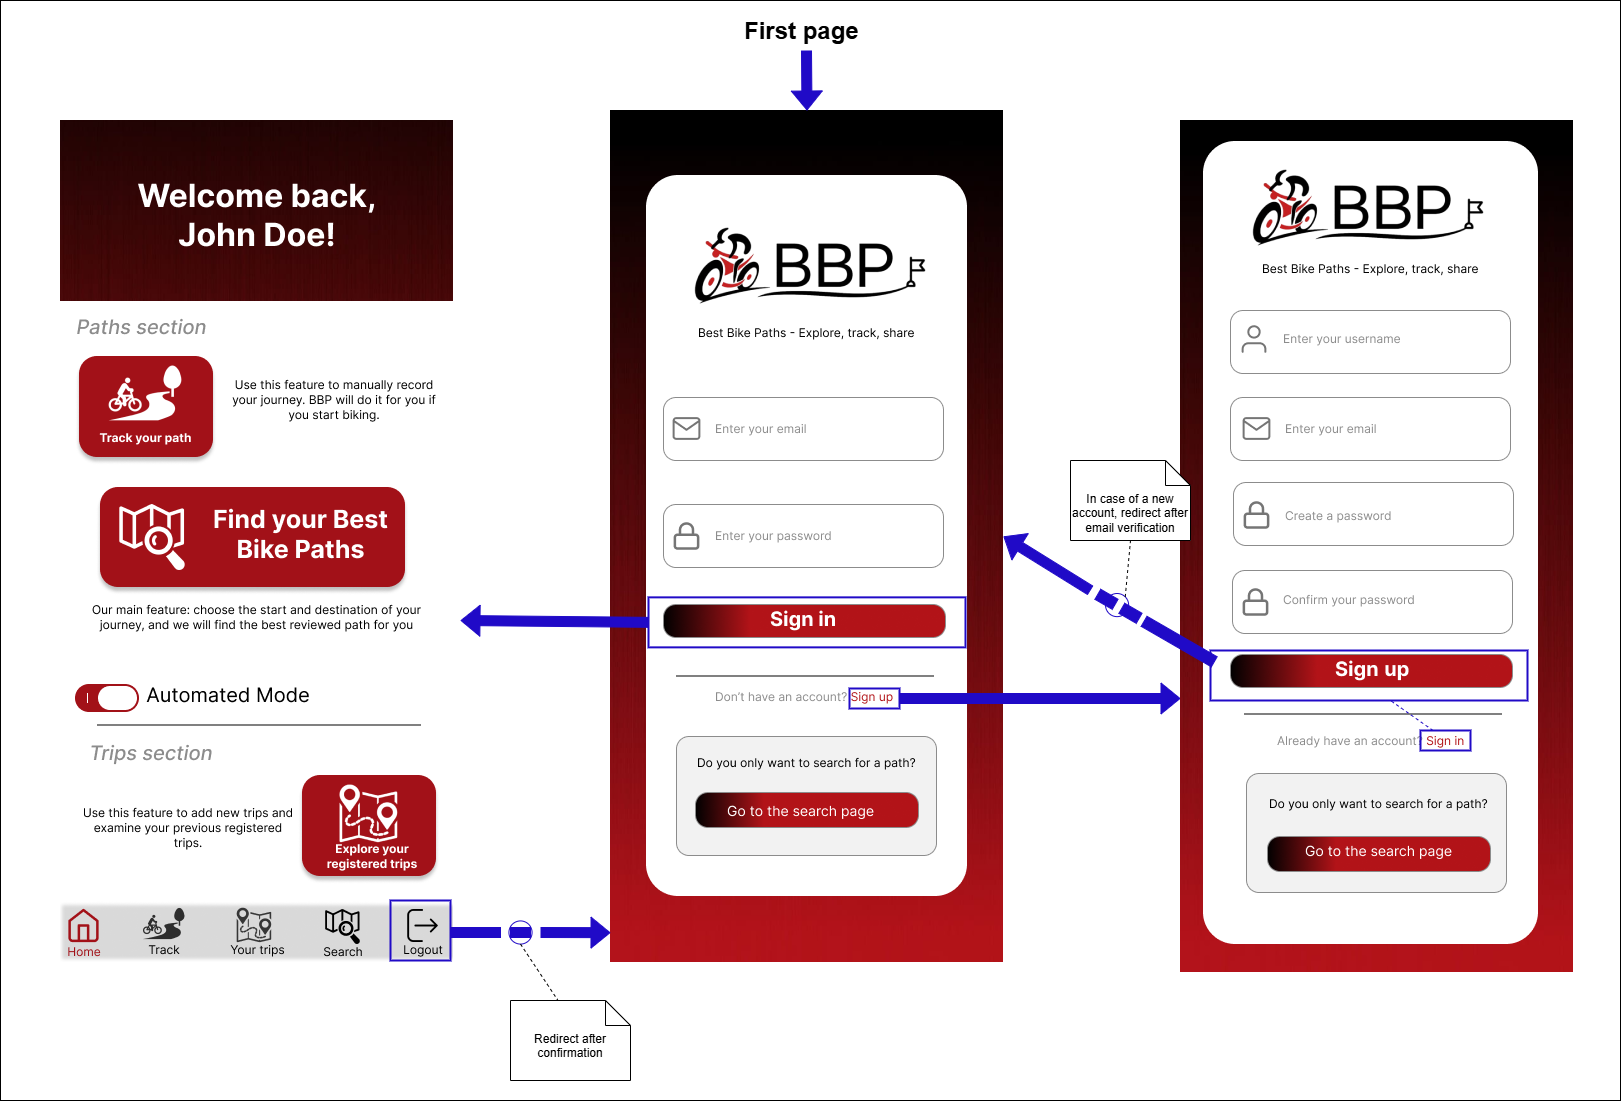
\includegraphics[width=\textwidth]{DD/Images/UI/Sign Up, Login, Logout.png}}
    \caption{Interaction between the pages regarding the sign up, log in and log out operations.}
\end{figure}

When the user opens the application, the Log In page is loaded. Here, the user can enter the system by providing their credentials and by pressing the "Sign In" button.\newline
If the user wants to register a new account, they can be redirected to the Sign Up page by pressing the "Sign up" text-button in the Log In page. Here the user can insert their information and, after an email verification process (not shown here for simplicity), successfully register into the system. After the process is completed, they are automatically redirected to the Log In page for their first login operation.\newline
If the user wants to delete their session data, they can log out from the system by pressing the "Logout" button at the bottom of the screen, where the Navigation Bar is located. They will be redirected to the Log In page.

\subsection*{Manual path tracking}
\begin{figure}[H]
    \fbox{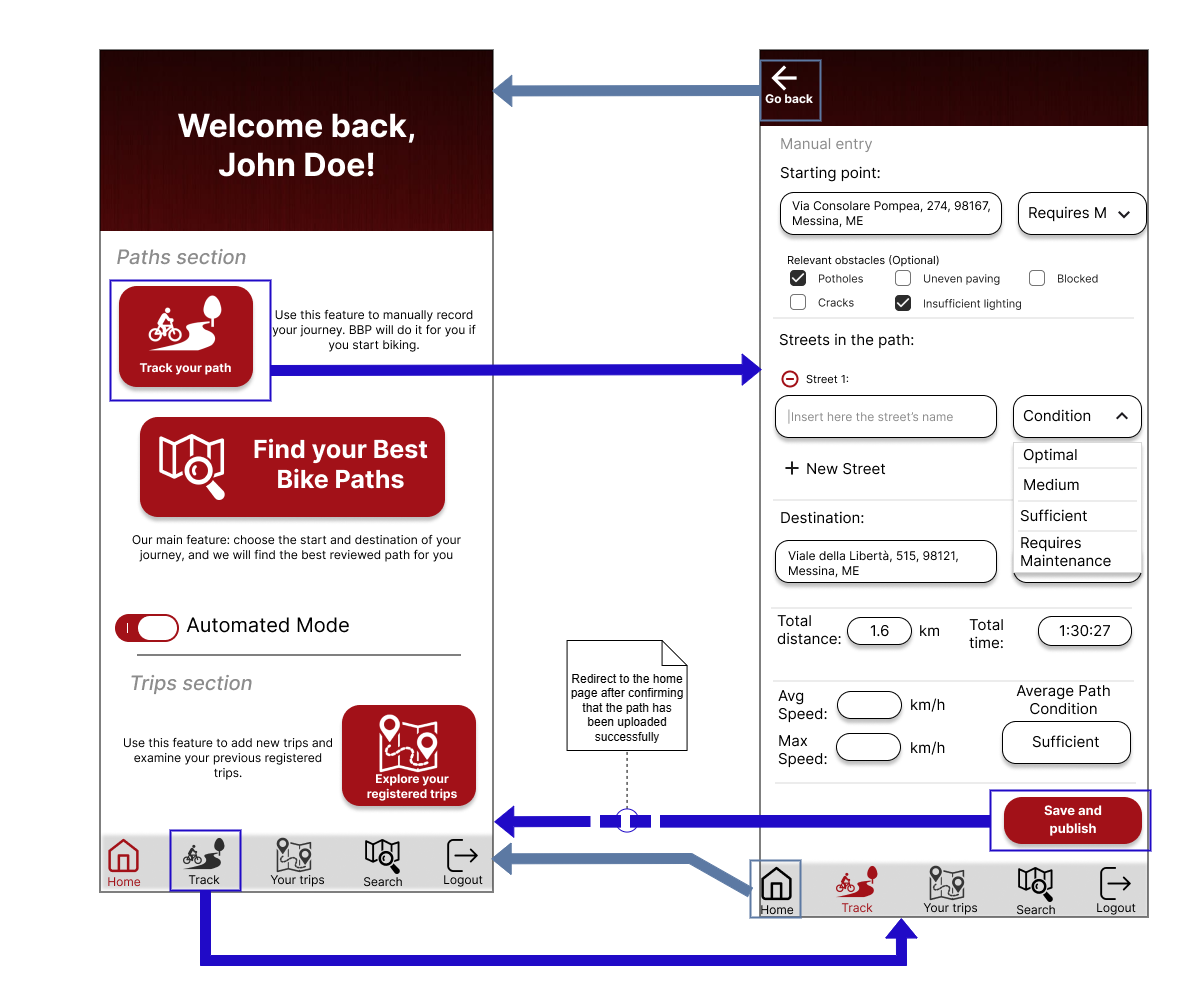
\includegraphics[width=\textwidth]{DD/Images/UI/Manual path tracking.png}}
    \caption{Interaction between the pages regarding the manual path tracking operation.}
\end{figure}

A registered user can easily access the manual path tracking by pressing the corresponding button in the home page or by pressing the track icon in the Navigation Bar, at the bottom of every page.\newline
Here the registered user must insert the starting and destination points of their bike path, and can, at any time, insert/remove another road between these two points by pressing the corresponding buttons.\newline
When the path needs to be registered into the system, the registered user can press the "Save and publish" button, successfully completing the operation. A notification is displayed to the registered user confirming the completion of the operation (not shown here for simplicity) and they are automatically redirected to the home page.\newline
At any point of the recording, the registered user can abort the procedure (and consequently clearing the fields) by pressing the "Go back" button at the top or the Home icon in the Navigation Bar.

\subsection*{Automated path tracking}
\begin{figure}[H]
    \fbox{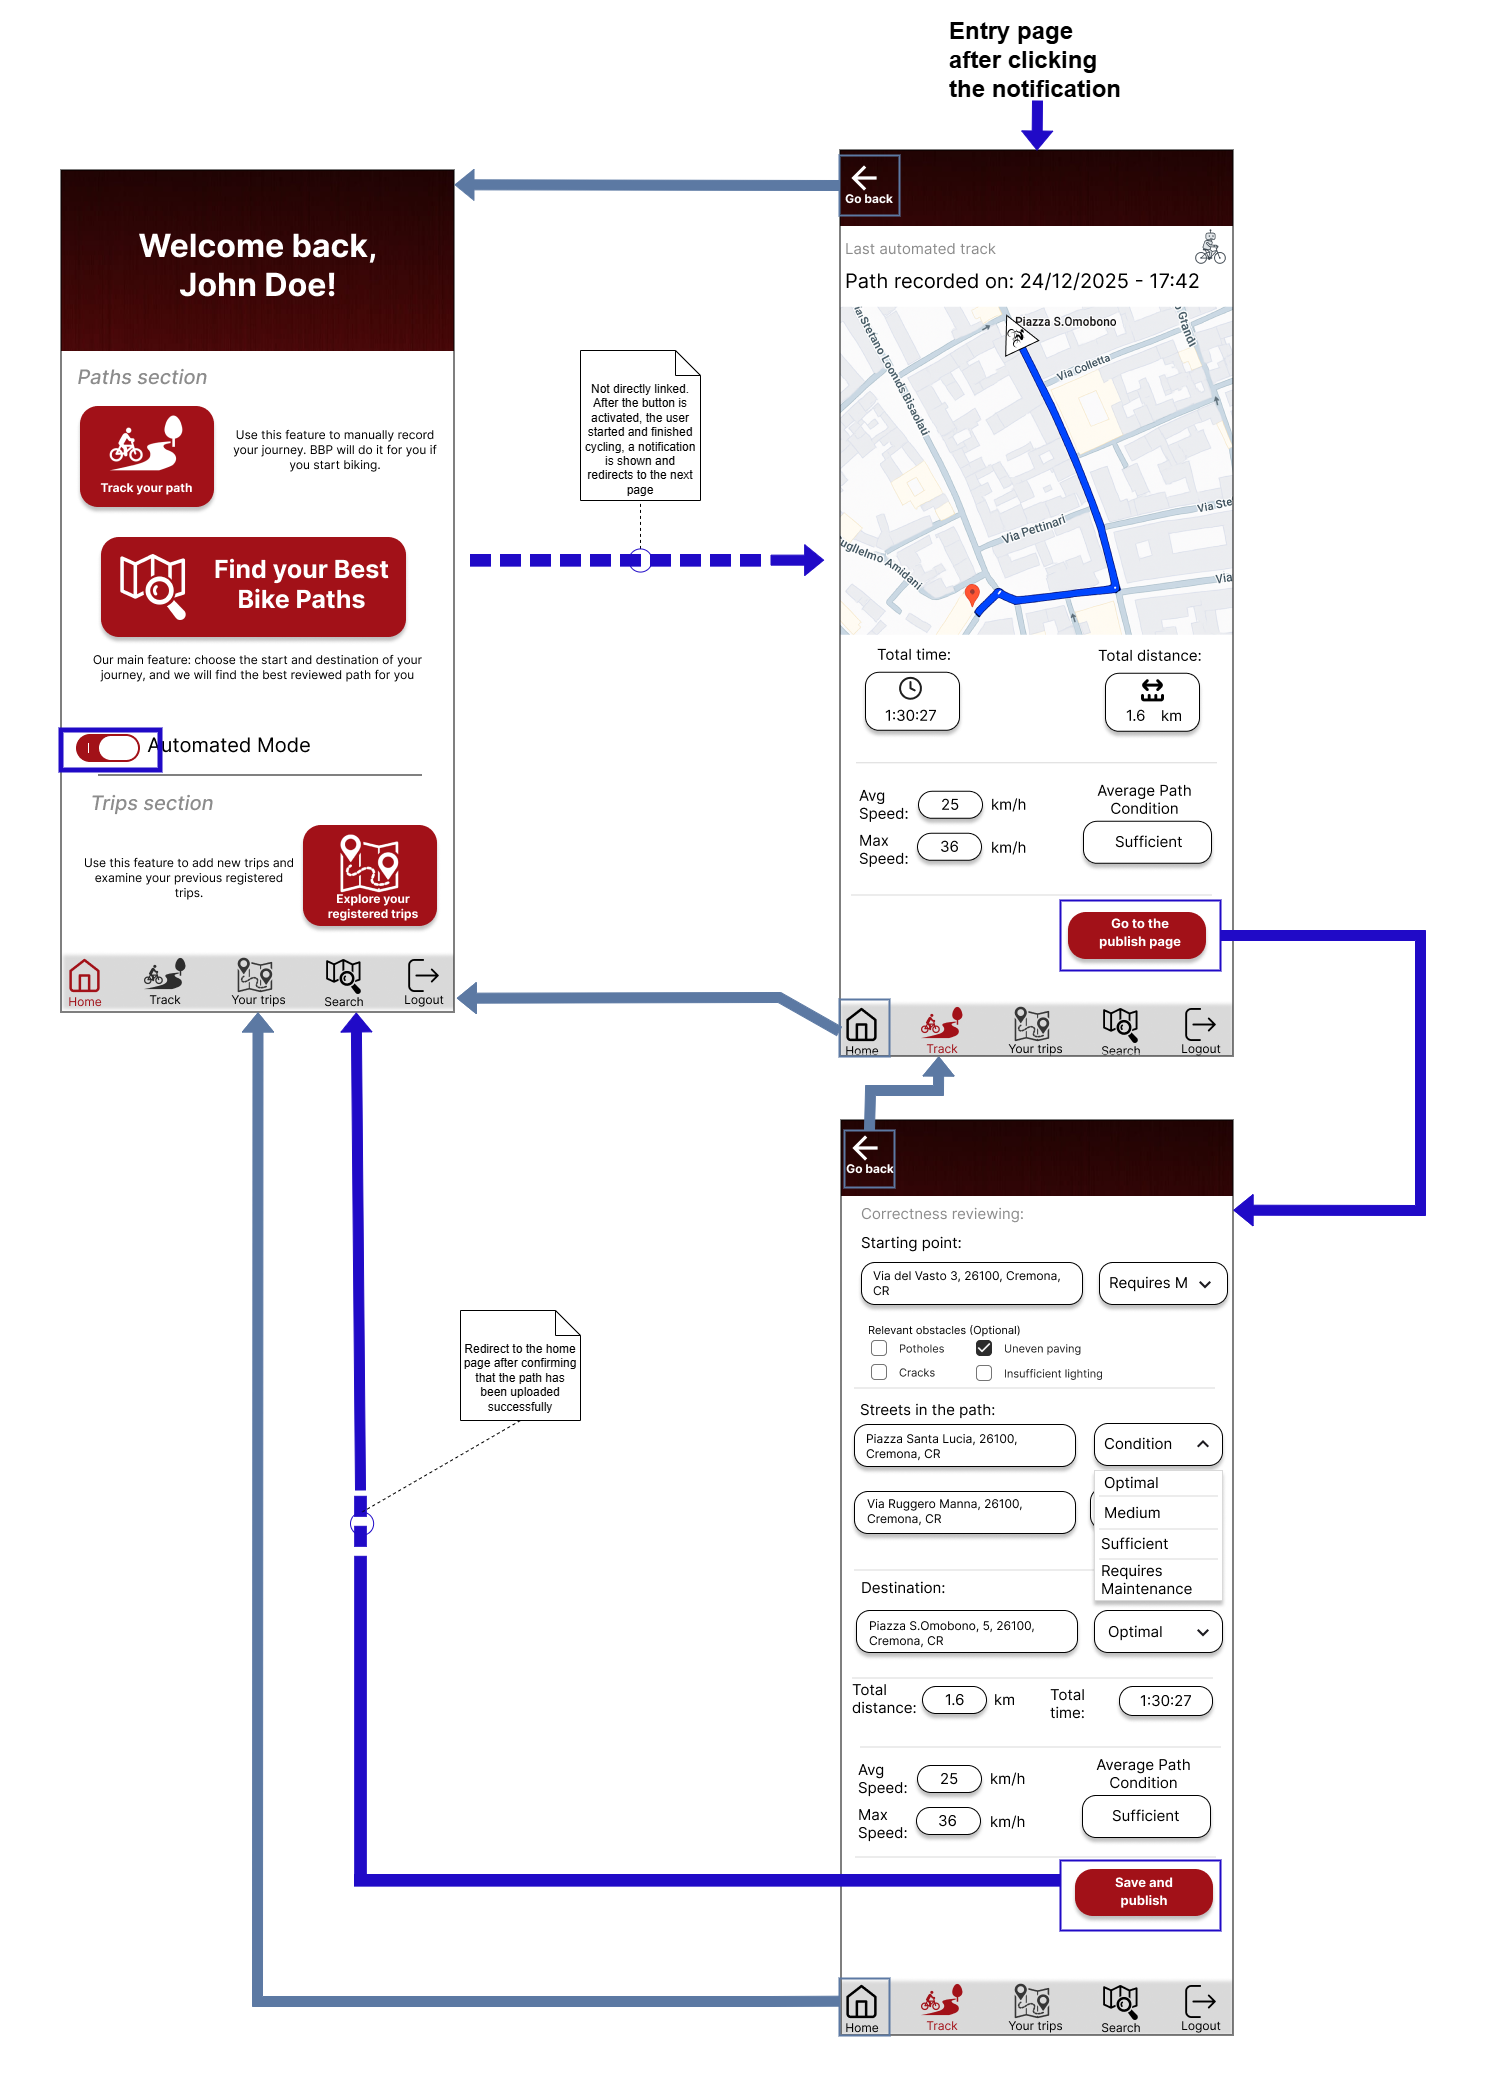
\includegraphics[width=\textwidth]{DD/Images/UI/Automated path tracking.png}}
    \caption{Interaction between the pages regarding the automated path tracking operation.}
\end{figure}

A registered user can track a path by using the automated mode, in which the application will access the sensors in the user's smartphone. To do so, the "Automated Mode" button must be activated.\newline
After the recording of a new path, a notification is displayed to the registered user, informing them that the recording was successful and it is ready to be reviewed. The registered user can see a summary of the recording by pressing the notification or opening the application. Here they can:
\begin{itemize}
    \item move on to the next step (the actual edit and review) by pressing the "Go to the publish page" button;
    \item or can discard the recording by pressing either the "Go back" button or the Home icon in the Navigation Bar.
\end{itemize}
The edit and publish page is very similar to the manual one, in which the registered user can adjust the content to their liking. When the path needs to be registered into the system, the registered user can press the "Save and publish" button, successfully completing the operation. A notification is displayed to the registered user confirming the completion of the operation (not shown here for simplicity) and they are automatically redirected to the home page.
\newline
At any moment, they can abort the operation by pressing the Home icon in the Navigation Bar or move back to the review page by pressing the "Go back" button.

\newpage
\subsection*{Trip recording and visualization}
\begin{figure}[H]
    \fbox{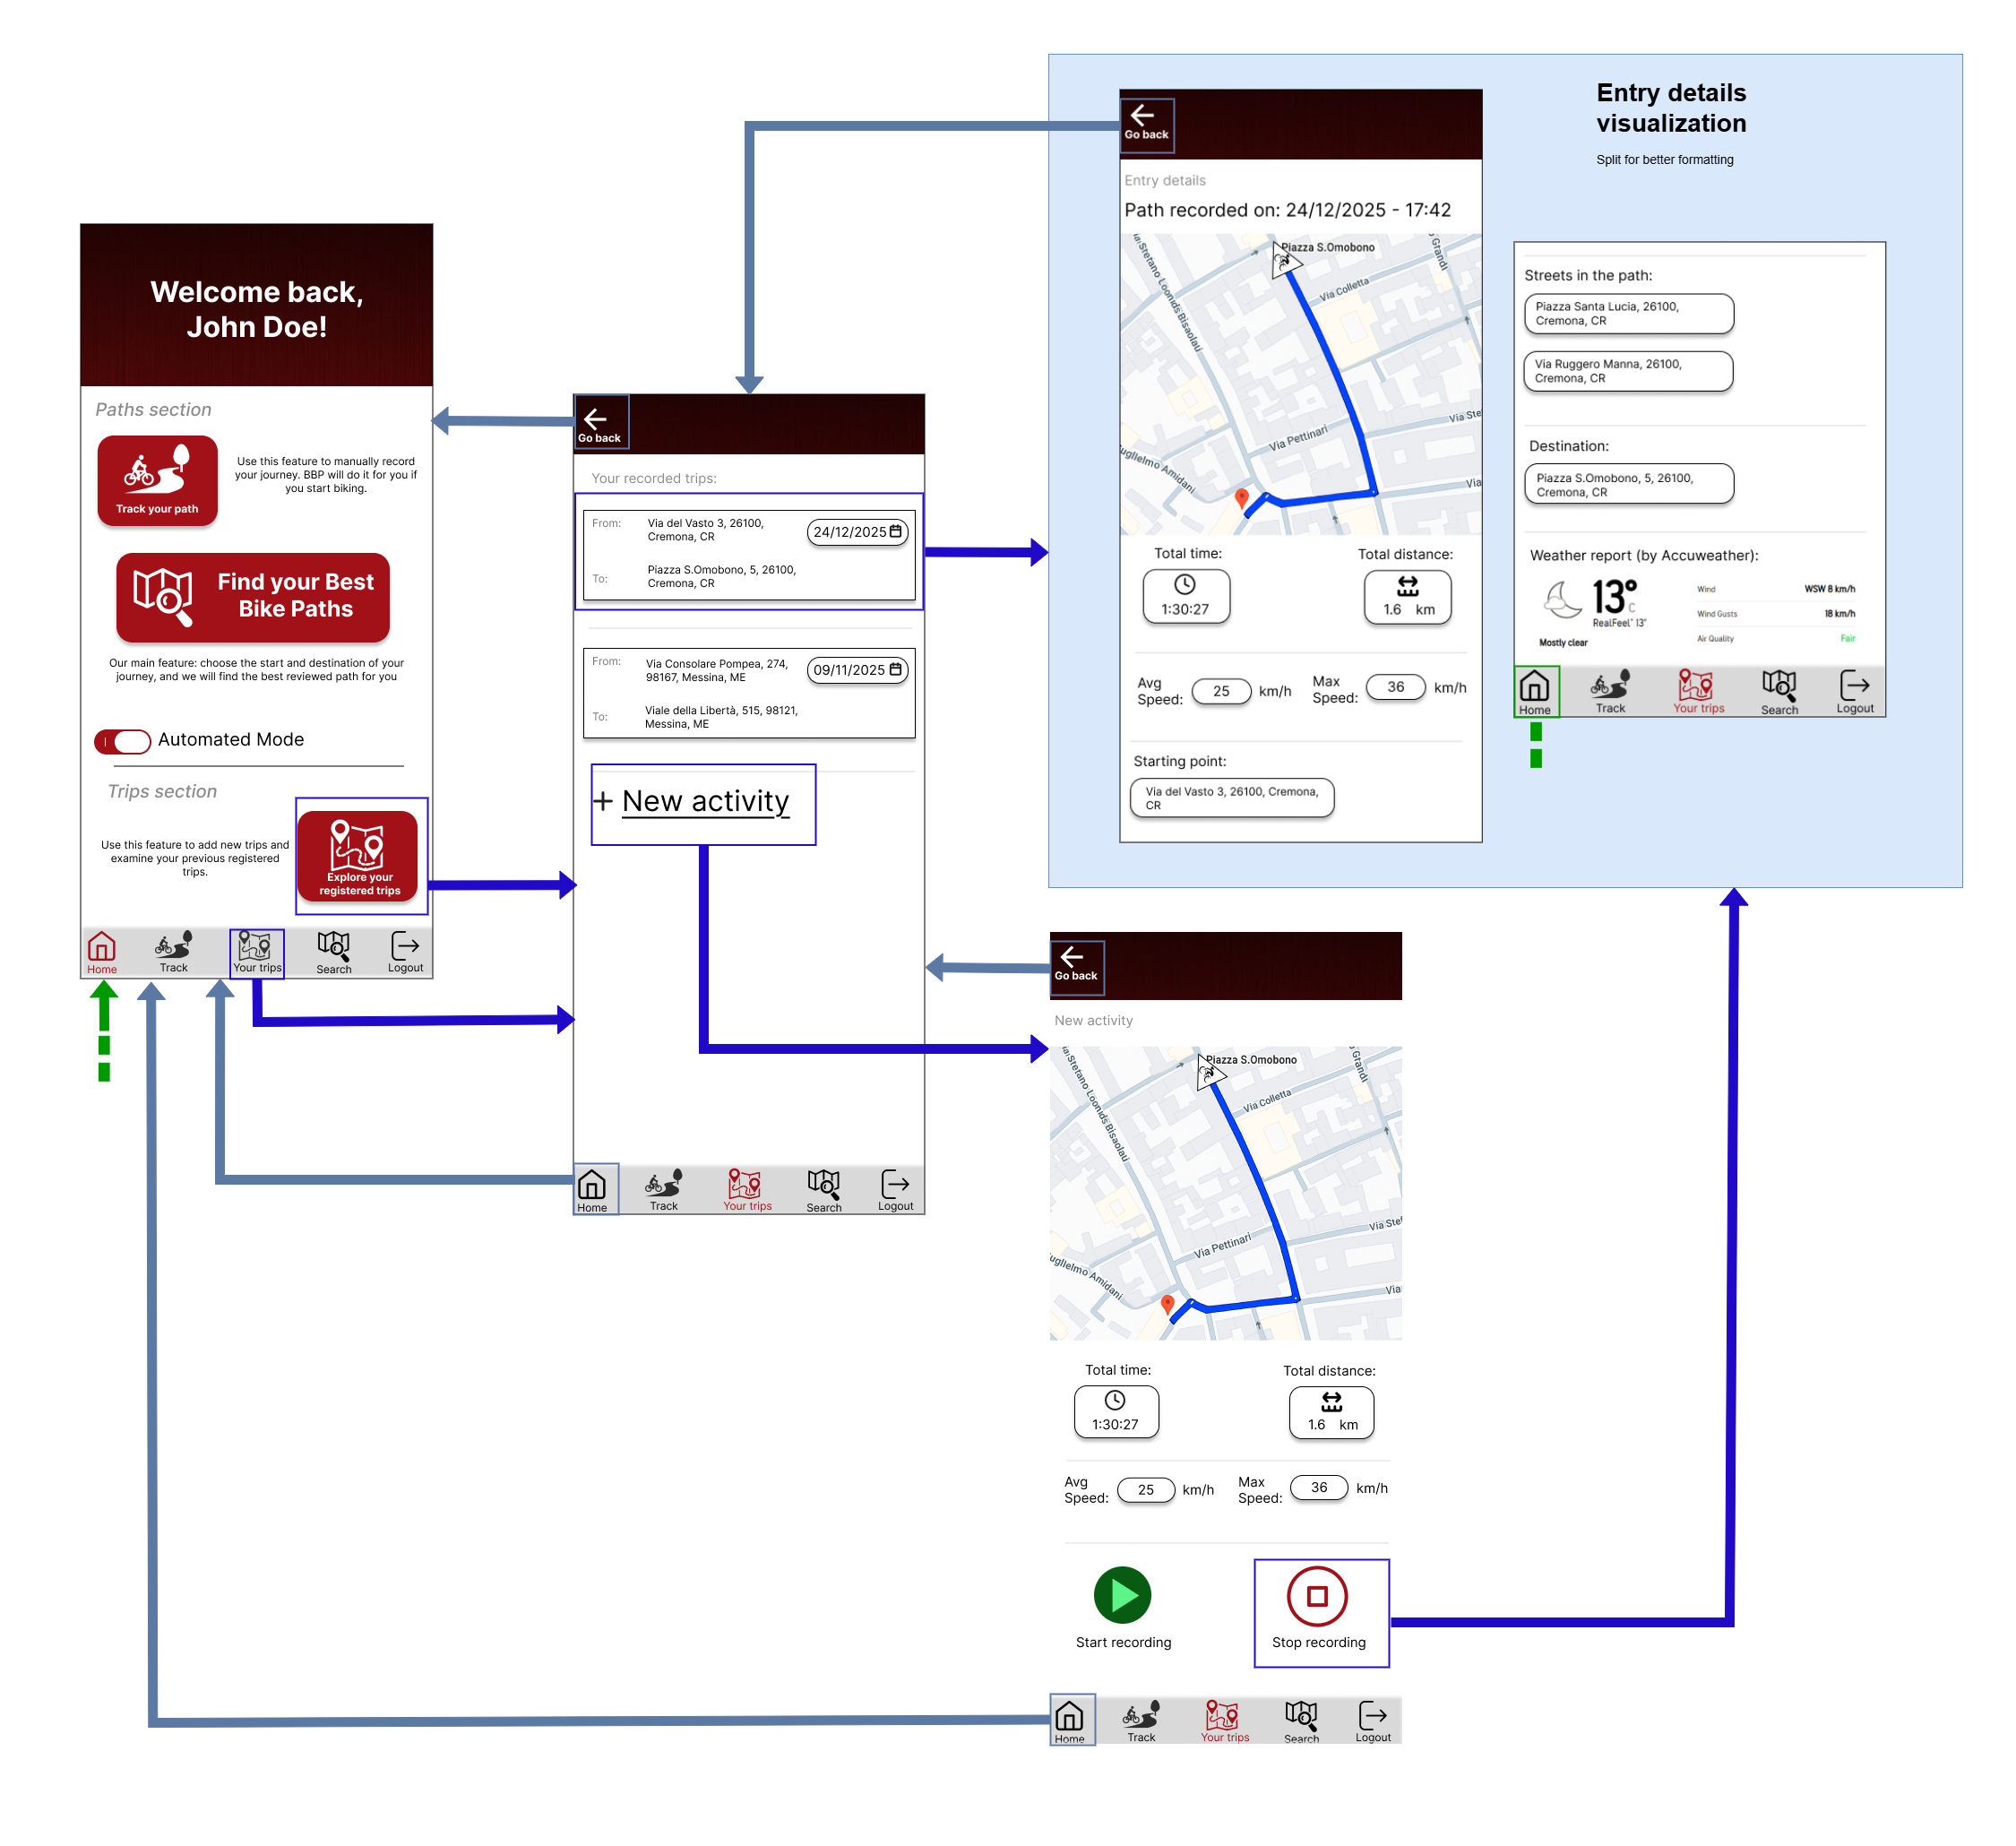
\includegraphics[width=\textwidth]{DD/Images/UI/Trips.png}}
    \caption{Interaction between the pages regarding the recording and visualization of trips (personal activities).}
\end{figure}
A registered user can track personal activities (or trips). To access the list of them, the registered user can press either the dedicated button "Explore your registered trips" or press the icon in the Navigation Bar.
\newline
Here, they are redirected into a new page, with the entire list of recorded activities. They can:
\begin{itemize}
    \item visualize an entry detail by pressing on it. Everything important is showed here, included performance metrics and weather details;
    \item start the recording of a new entry by pressing on the text-button "New activity". They are redirected to a new page, in which the registered user can start, pause and stop the recording, while important metrics are visualized. After the registered user is ready to save the new activity, they can press the "Stop recording" button and, after a notification confirming the successful operation is displayed, they are redirected to the entry details page.
\end{itemize}
In each of the steps, the user can move back to the previous page or use the navigation bar.
\newpage
\subsection*{Best Bike Paths search engine}
\begin{figure}[H]
    \fbox{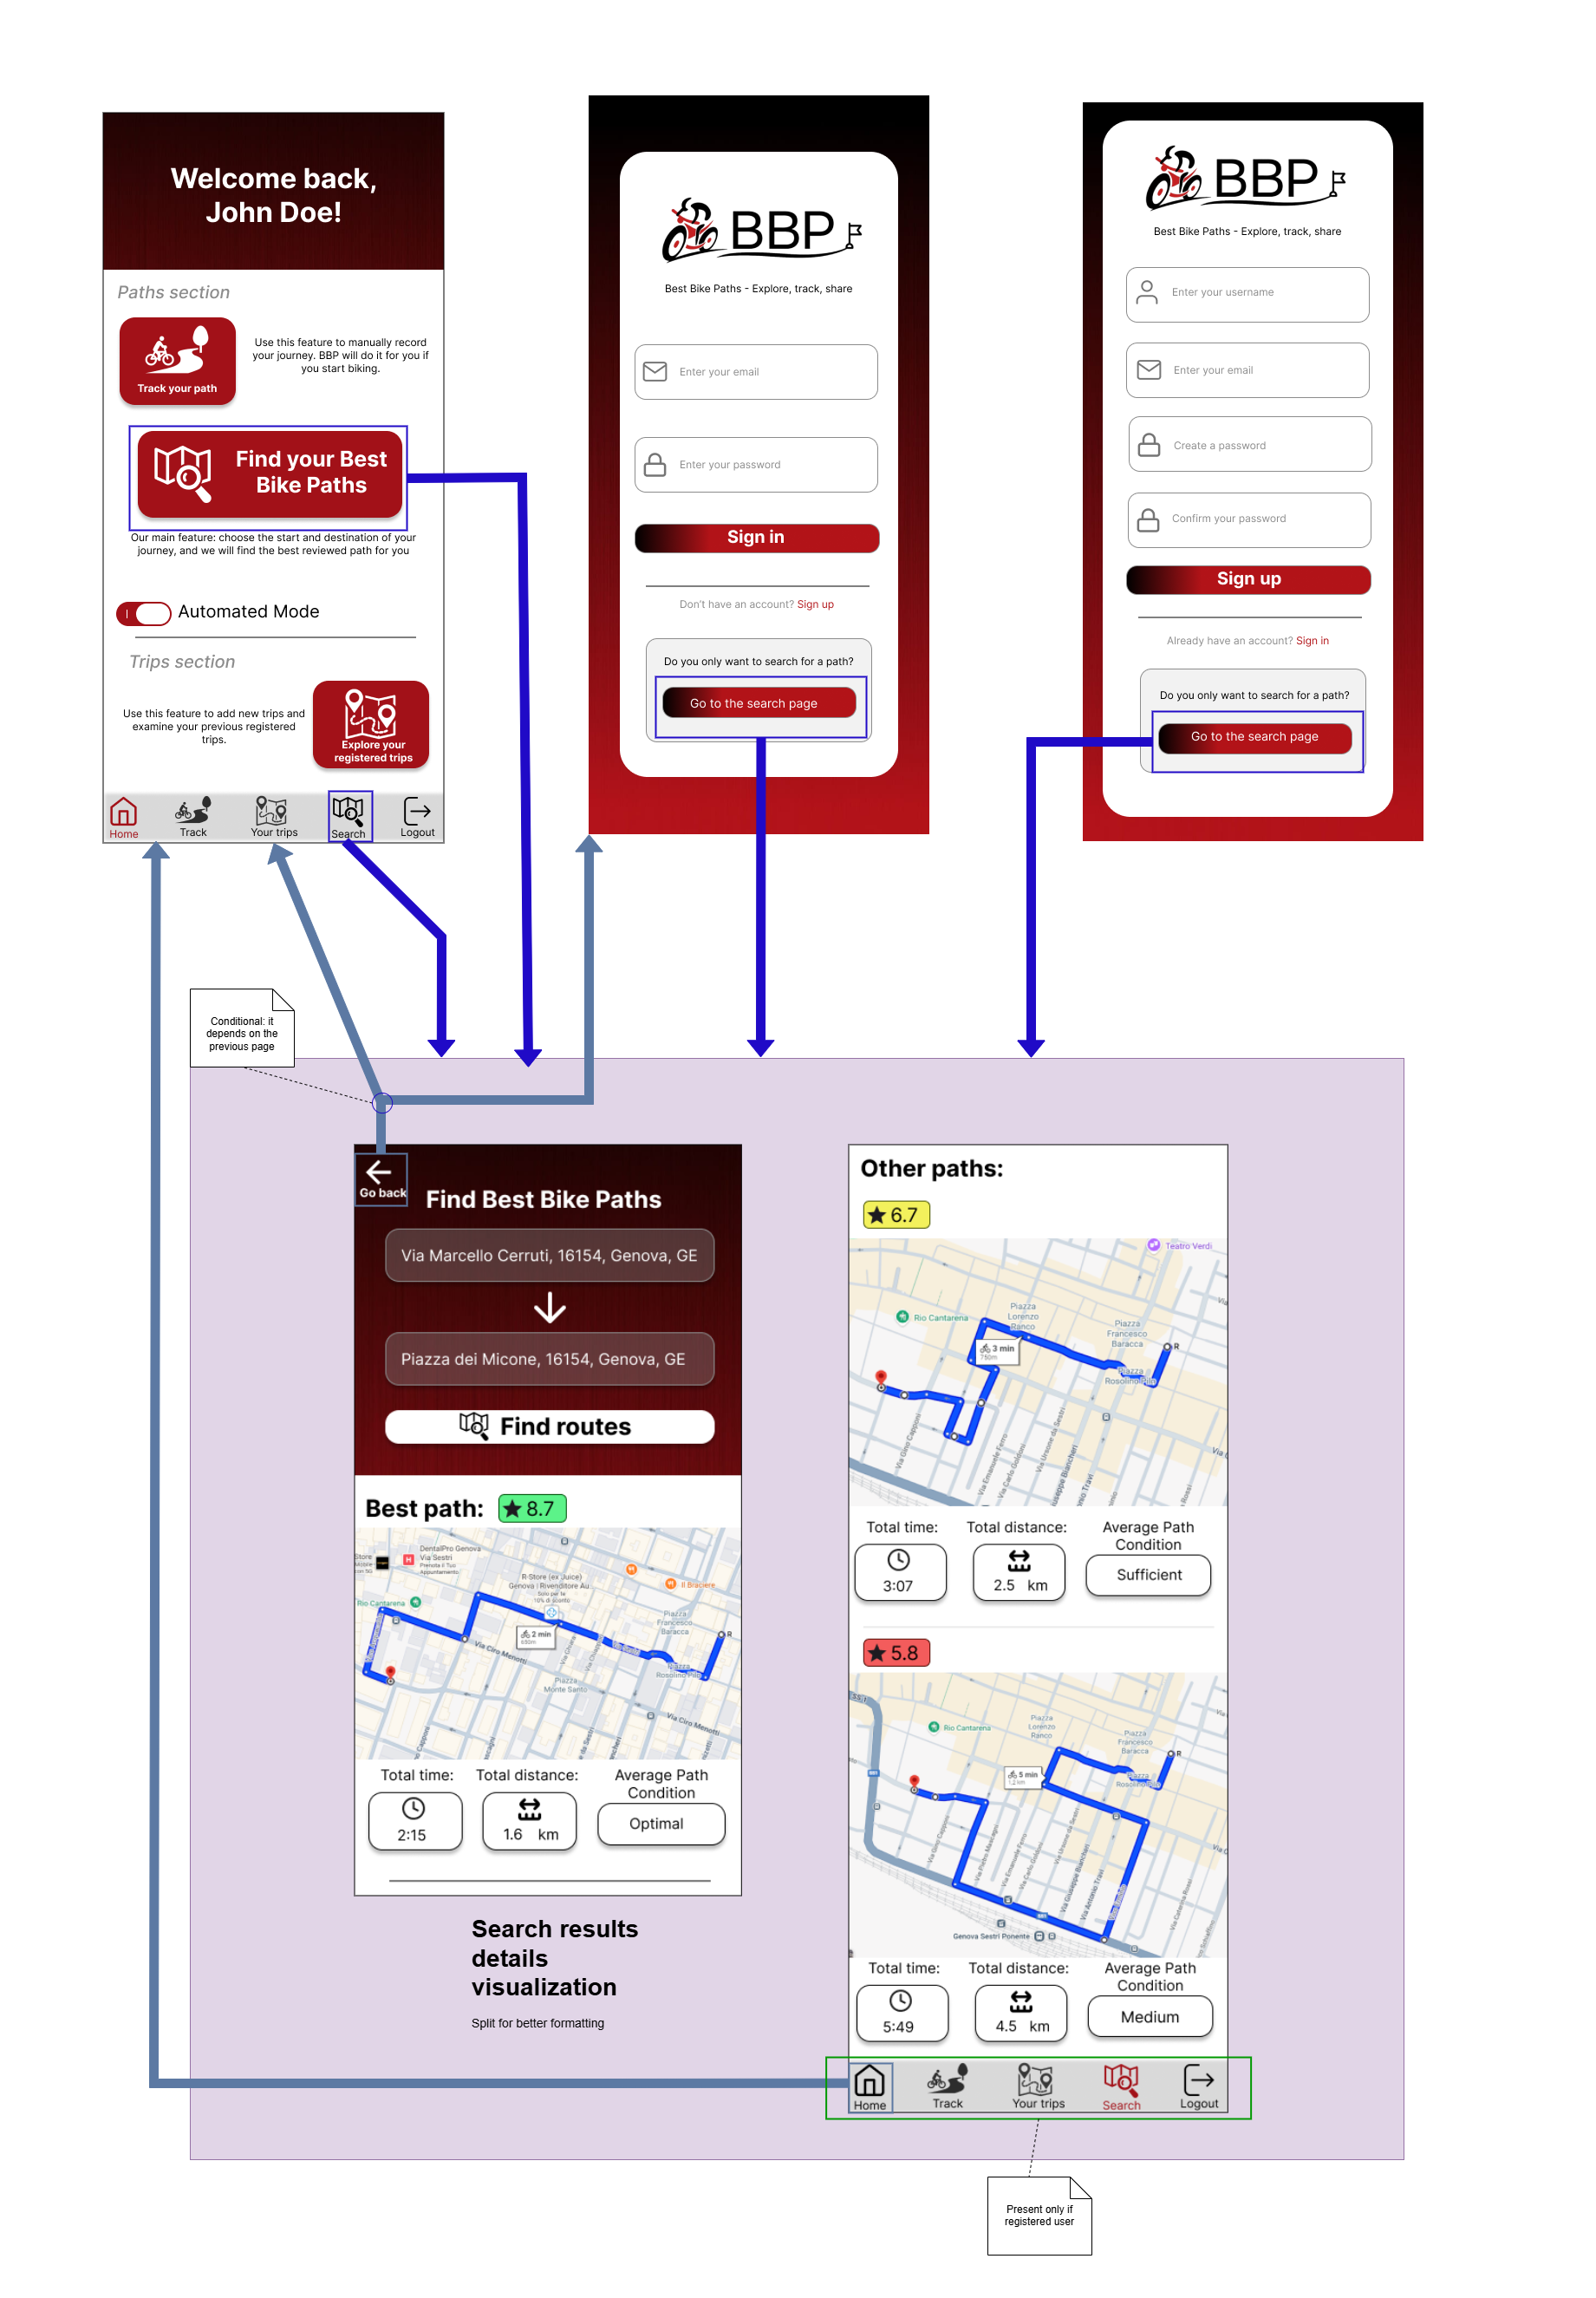
\includegraphics[width=0.97\textwidth]{DD/Images/UI/BBP search engine.png}}
    \caption{Interaction between the pages regarding the search of possible paths.}
\end{figure}
 Any user (either registered or not) can search for the possible best bike path(s) using BBP system. To do so, they can access the search engine page by pressing either:
 \begin{itemize}[label = -]
    \item the dedicated button in the home page (registered user only);
    \item the dedicated icon in the Navigation Bar (registered user only);
    \item the "Go to the search page" buttons in the Log In and Sign Up pages.
\end{itemize}
Here the user can, by inserting source and destination locations, search for the best possible bike path(s) between two points. If more than one is present in the database, the application will show them based on a calculated score.\newline
In any moment, they can go back to the previous page (either the home page or the log in page) and, for registered users only, use the navigation bar.

\subsection*{Final notes on Navigation Bar}
In each page after the Log In, the Navigation Bar is present and can be used to access specific pages. This guarantees easy access and fast navigation through the pages.

\begin{figure}[H]
    \fbox{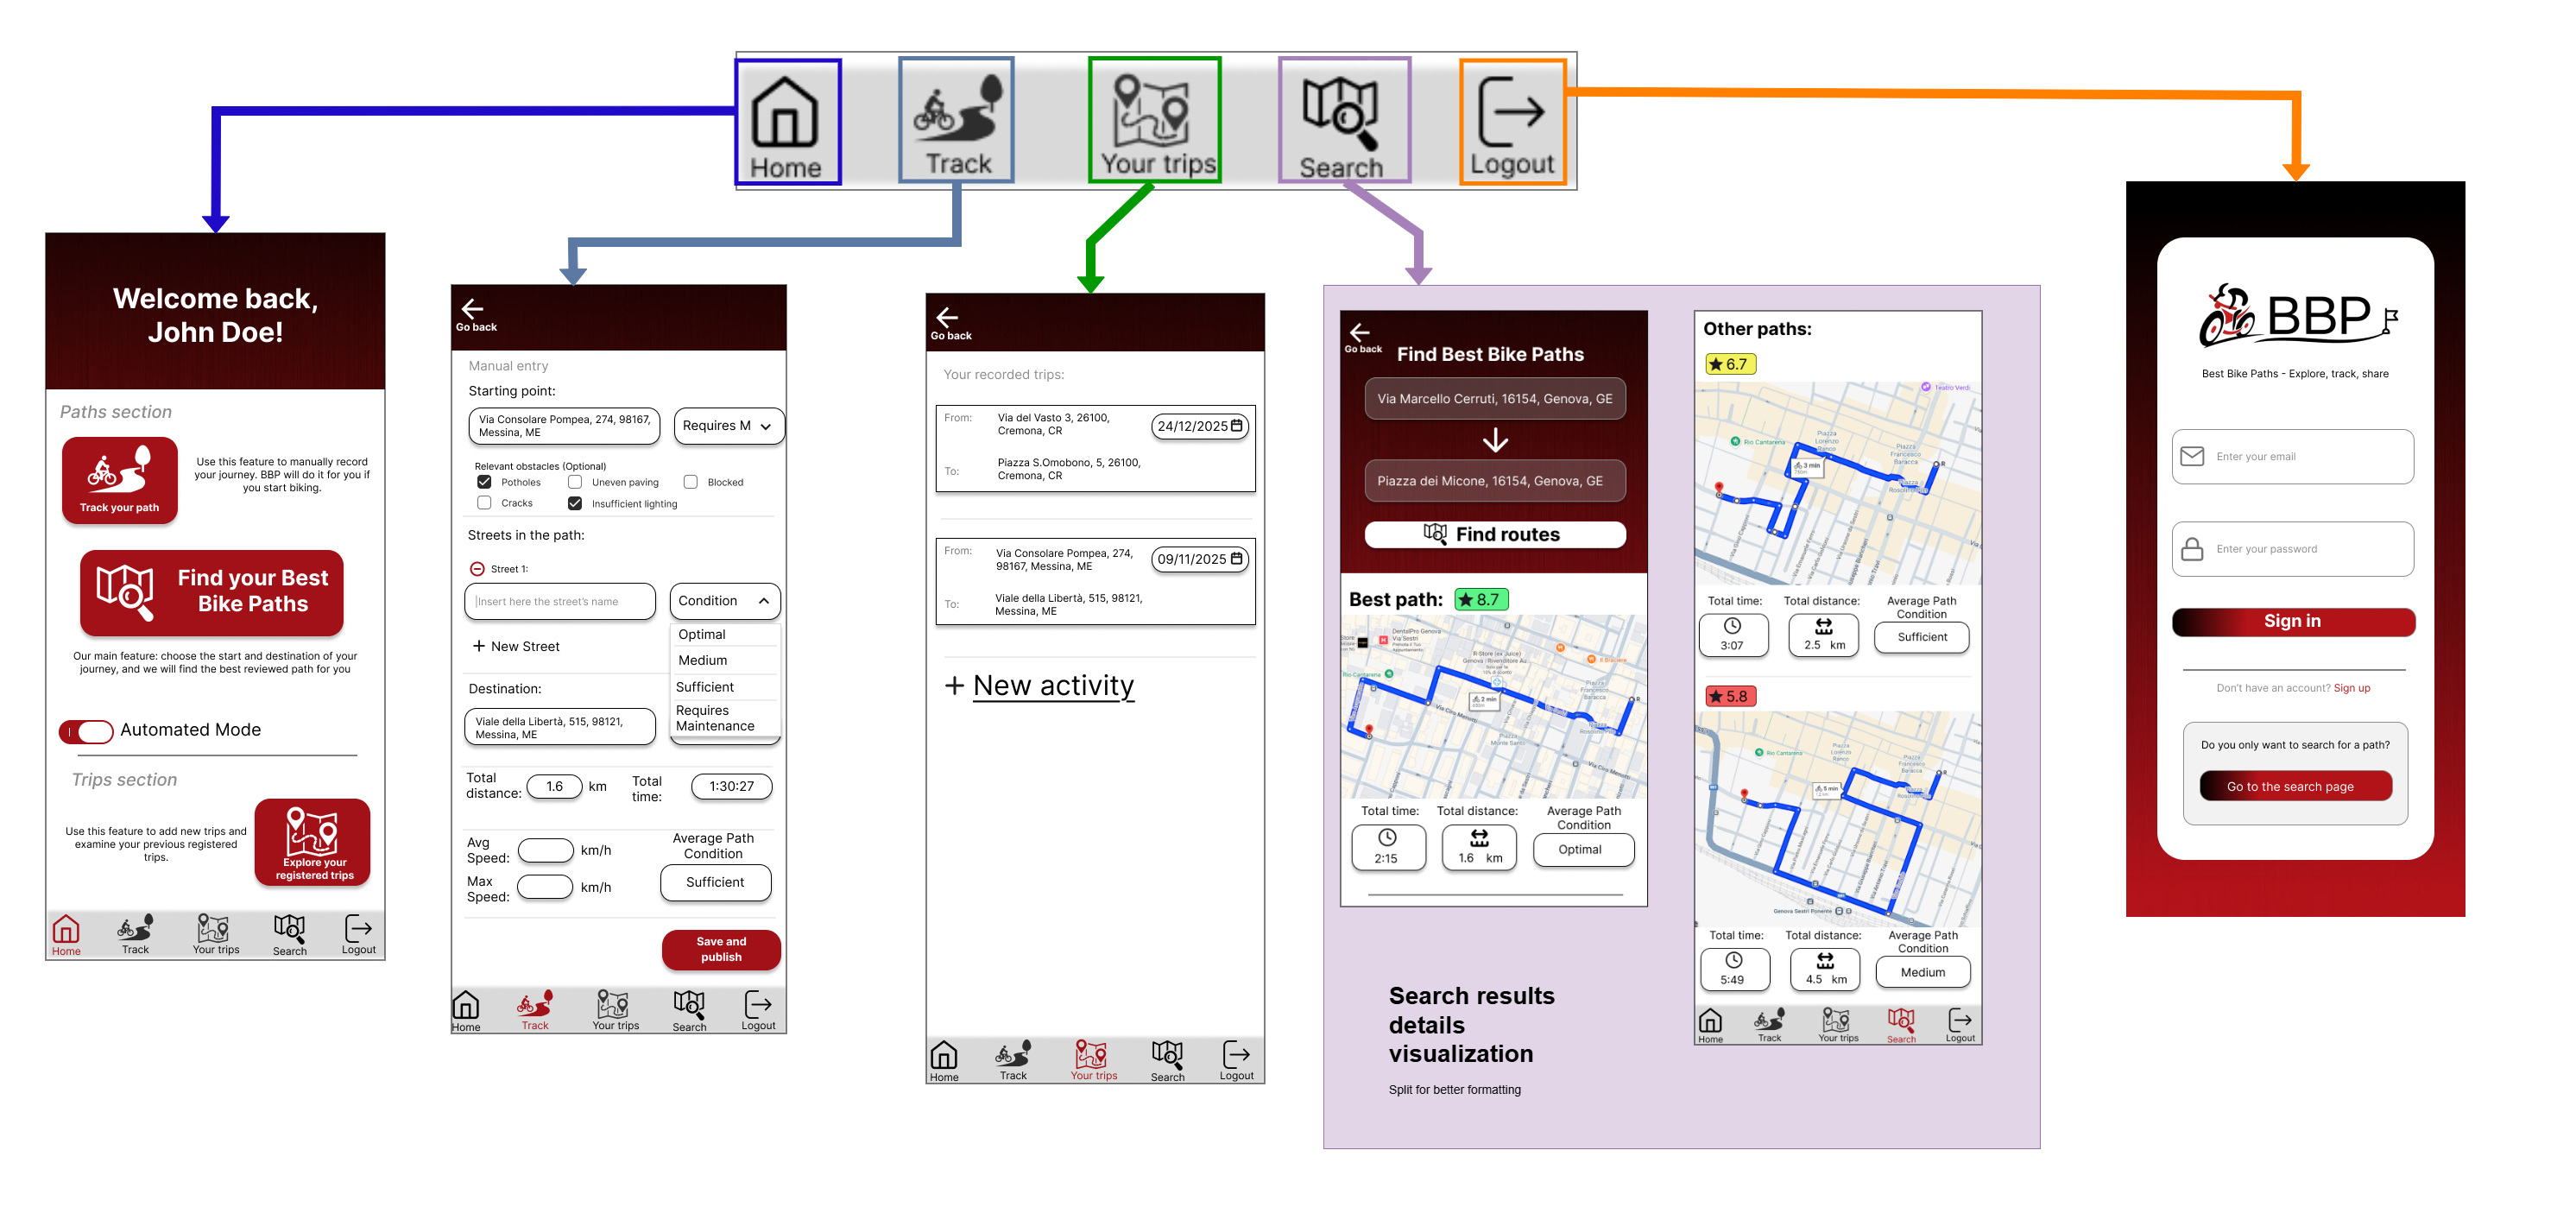
\includegraphics[width=0.97\textwidth]{DD/Images/UI/Navigation Bar.png}}
    \caption{Navigation Bar links.}
\end{figure}